% Figure snippets for main.tex — do NOT \input{} this; embed inline.

% Figure: validation placeholder (representative micrographs unavailable in extraction)
\begin{figure}[htbp]
\centering
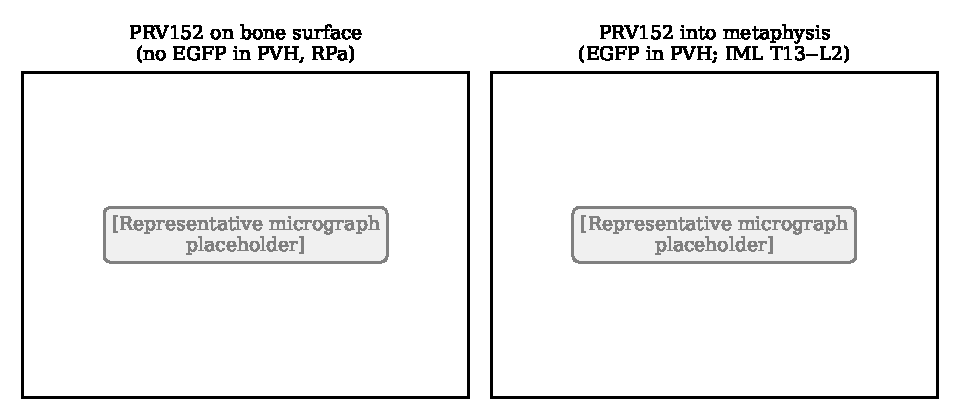
\includegraphics[width=0.78\textwidth]{figures/fig_validation.pdf}
\caption{Validation of PRV152 transneuronal tracing. Left: when PRV152 was placed on the bone surface, no EGFP signal was detected in the paraventricular hypothalamic nucleus (PVH) or the raphe pallidus (RPa). Right: PRV152 injection into the periosteum or metaphysis produced EGFP-immunoreactive neurons in the PVH, and PRV152-labeled neurons were detected in the intermediolateral cell column (IML) of the spinal cord at T13--L2, consistent with the expected bone--SNS ganglia--IML--brain route. Panels are placeholders; representative micrographs are unavailable in the provided extraction. Scale bar corresponds to 50\,$\mu$m in the source images.}
\label{fig:validation}
\end{figure}

% Figure: per-division counts (data-grounded)
\begin{figure}[htbp]
\centering
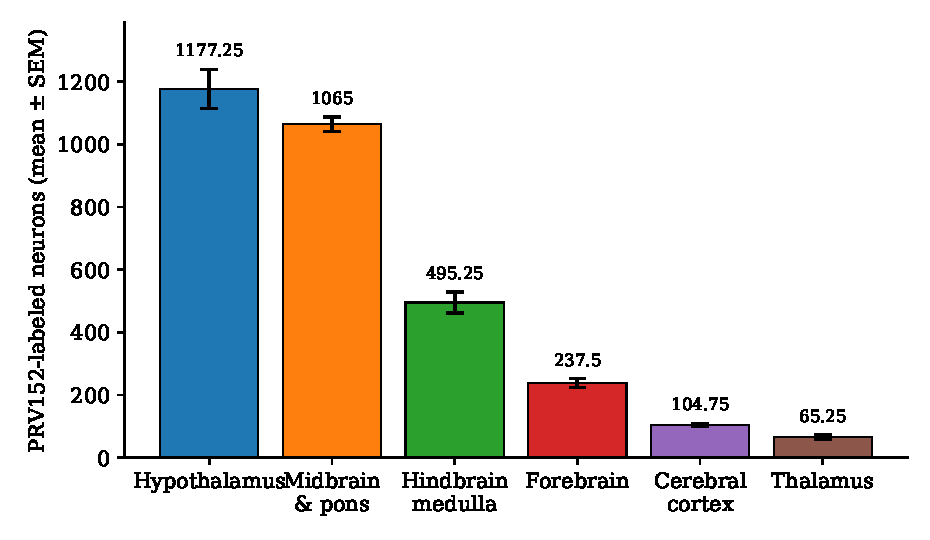
\includegraphics[width=0.82\textwidth]{figures/fig_counts.pdf}
\caption{PRV152-labeled neurons summed across each of six brain divisions after right-femur PRV152 injection (mean $\pm$ SEM, $N=4$ analyzable mice). The hypothalamus contains the most labeled neurons ($1177.25 \pm 62.75$), followed by midbrain and pons ($1065 \pm 22.39$), hindbrain medulla ($495.25 \pm 33.49$), forebrain ($237.5 \pm 15.08$), cerebral cortex ($104.75 \pm 4.64$) and thalamus ($65.25 \pm 7.78$). Error bars are SEM.}
\label{fig:counts}
\end{figure}

% Figure: number of positive sub-regions per division (data-grounded)
\begin{figure}[htbp]
\centering
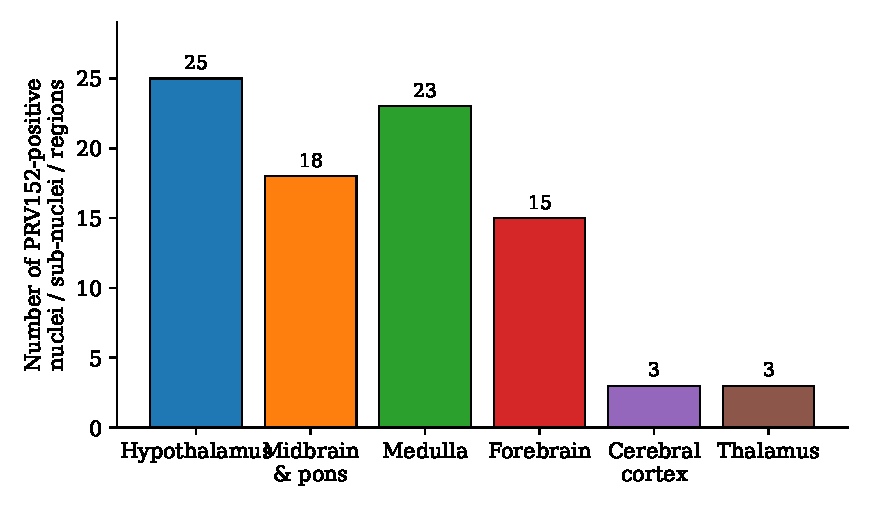
\includegraphics[width=0.75\textwidth]{figures/fig_subnuclei.pdf}
\caption{Number of PRV152-positive nuclei, sub-nuclei, and regions identified within each brain division. The hypothalamus, medulla and midbrain/pons each span more than a dozen distinct labeled structures, whereas the cerebral cortex and thalamus each contributed three labeled regions.}
\label{fig:subnuclei}
\end{figure}

% Figure: schematic circuit (schematic)
\begin{figure}[htbp]
\centering
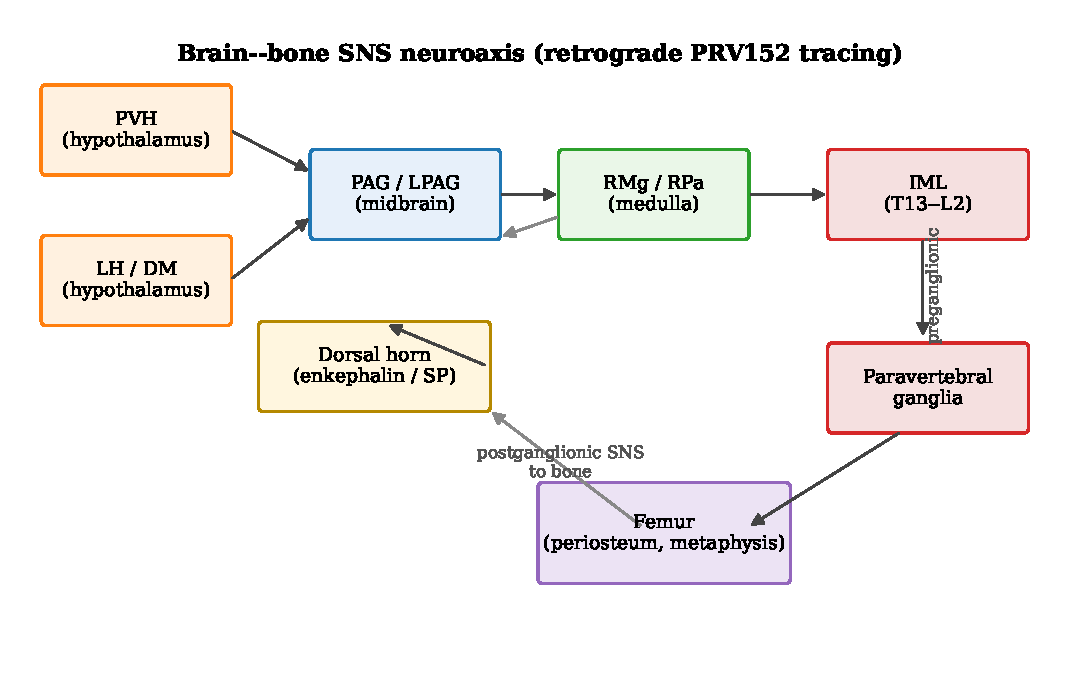
\includegraphics[width=0.92\textwidth]{figures/fig_circuit.pdf}
\caption{Schematic of the candidate central SNS brain--bone neuroaxis inferred from the current PRV152 dataset together with prior adipose-depot and marrow tracing. Pre-autonomic neurons of the hypothalamic paraventricular nucleus (PVH), together with lateral and dorsomedial hypothalamus (LH/DM), project to periaqueductal gray (PAG/LPAG) neurons of the midbrain. The PAG interfaces with the medullary raphe magnus and raphe pallidus (RMg/RPa), which deliver descending projections to the dorsal horn, where they regulate enkephalinergic control of substance P-mediated pain transmission. Sympathetic outflow reaches the femur via preganglionic neurons in the intermediolateral cell column at T13--L2, then paravertebral chain ganglia, and finally postganglionic SNS fibers that innervate periosteum and metaphyseal bone.}
\label{fig:circuit}
\end{figure}
